\section{Durchführung}
\label{sec:Durchführung}
Der Versuch besteht im wesentlichen aus einem Lock-In-Verstärker und einem Oszilloskop. Außerdem wird für den zweiten Versuchsteil eine Leuchtdiode und ein Photodetektor benötigt.
Für den ersten Versuchsteil wird die Schaltung, wie in Abbildung \ref{fig:aufa} zu sehen ist, aufgebaut.
\begin{figure}
    \centering
    \caption{Schematischer Aufbau eines Lock-In-Verstärkers mit Rausch Generator.\cite{v303}}
    \label{fig:aufa}
    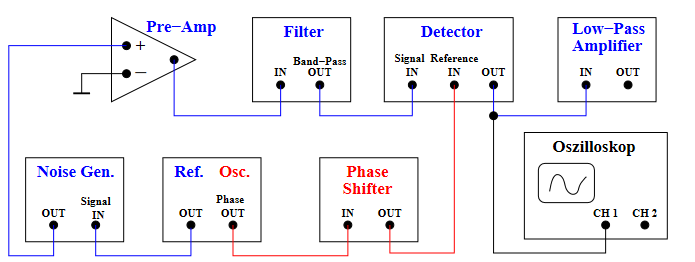
\includegraphics[width = 0.6 \textwidth]{Pics/aufa.png}
\end{figure}
Dabei wird zunächst der Rausch Generator überbrückt. Es werden sechs verschiedene Phasen am Phasenverschieber eingestellt und die entstehenden
Bilder werden am Oszilloskop gespeichert. Das Verfahren wird noch einmal mit dem angeschlossenen Rausch Generator durchgeführt.
\\
Für den zweiten Aufgabenteil wird, wie in Abbildung \ref{fig:aufb} zu sehen ist, an der Stelle des Rausch Generators eine LED und ein Photodetektor im Abstand $r$ von einander angeschlossen.
Dabei ist der Abstand variierbar. 
\begin{figure}
    \centering
    \caption{Schematischer Aufbau eines Lock-In-Verstärkers mit Leuchtdiode und Photodetektor.\cite{v303}}
    \label{fig:aufb}
    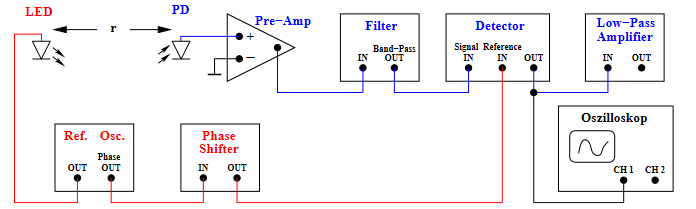
\includegraphics[width = 0.6 \textwidth]{Pics/aufb.png}
\end{figure}
Es werden 15 bis 20 mal die Wertepaare des Abstands und der davon abhängigen Spannungsamplitude bestimmt.